\subsection{ODE tests}
In this section, we will apply the introduced explicit, implicit and IMEX methods on ordinary differential equations to compare them with the theoretical results obtained before. Remark that our implementation takes usage of the linearized versions as in \eqref{eq: L1_linearized_ADER}. This is exact for linear systems, but has to be kept in mind while considering nonlinear ODEs. 
\subsubsection{Validation of the ImsDeC stability region}
%\begin{figure}[!h]
%	\centering
%	\includegraphics[width=0.65\textwidth]{odepics/BspImsDeC/IMsDeC11_GLB.png}
%	\caption{Stability Region for ImsDeC11 with Gauss-Lobatto nodes}
%	\label{fig: stabreg_ImsDeC11_GLB}
%\end{figure}
As seen in Figures~\ref{fig: ODEIMDeCADER} and \ref{fig: exaImsDeC_high}, the ImsDeC has an unexpected behavior by being the only considered pure implicit method here, which does not possess the almost A-stability for higher orders. We want to review this by applying the method on ODEs. \\
As example we take the ImsDeC11 with Gauss-Lobatto nodes, because it has the smallest stability region out of all ImsDeC methods. We observe that the limited, stable region has its left border approximately at $z=900+0i$. \\
Solving at first the linear, scalar ODE
\begin{equation}\label{eq: ImsDeC_linear_scalar}
\partial_t y(t) =-10^3y(t), y(0)=1,
\end{equation}
with different step sizes $h_1=1.0, h_2=0.5, h_3=0.02, h_4=0.01$, we expect the ImsDeC method for $h_1$ to be unstable and for the remaining 3 $h_i$ to be stable, because 
\begin{align*}
&z_1=\lambda\cdot h_1=-10^3\cdot 1=-10^3 \notin S,\\
&z_i=\lambda\cdot h_i>-900 \in S,\quad i\in\{2,3,4\},
\end{align*}
where $S$ denotes the stability region of the ImsDeC11 with Gauss-Lobatto nodes. The numerical results are shown in figure~\ref{fig: exaImsDeC1}. We observe that for $h_1$, the method diverges from the decaying exact solution $y(t)=e^{-10^3t}$, which is in agreement with $z_1 \notin S$. In the second case for $h_2$, we see the solution curve mimicking the decaying behavior, which coincides having $z_2\in S$. As a comparison, we also plot the ImDeC11 with Gauss-Lobatto nodes which is known as almost A-stable and shows appropriate results. As seen in figure~\ref{fig: exaImsDeC2}, of course for both $z_3$ and $z_4$, we obtain qualitative good solutions. 
We also display the sDeC11 in these figures and observe that their stability properties are still much worse than these of the ImsDeC11, as its stability region ends around $z\approx 6$, which make $h_c=\frac{6}{10^3}$ the threshold for a stable discretization.

We can summarize that the numerically calculated stability regions are validated through this experiment. 
Notice further that the linearization of the implicit method does not influence the stability contrary in that case. \todo{what does this line mean? I do not know.. we should reried it..}
\begin{figure}
	\centering
	\begin{minipage}[t]{0.45\textwidth}
		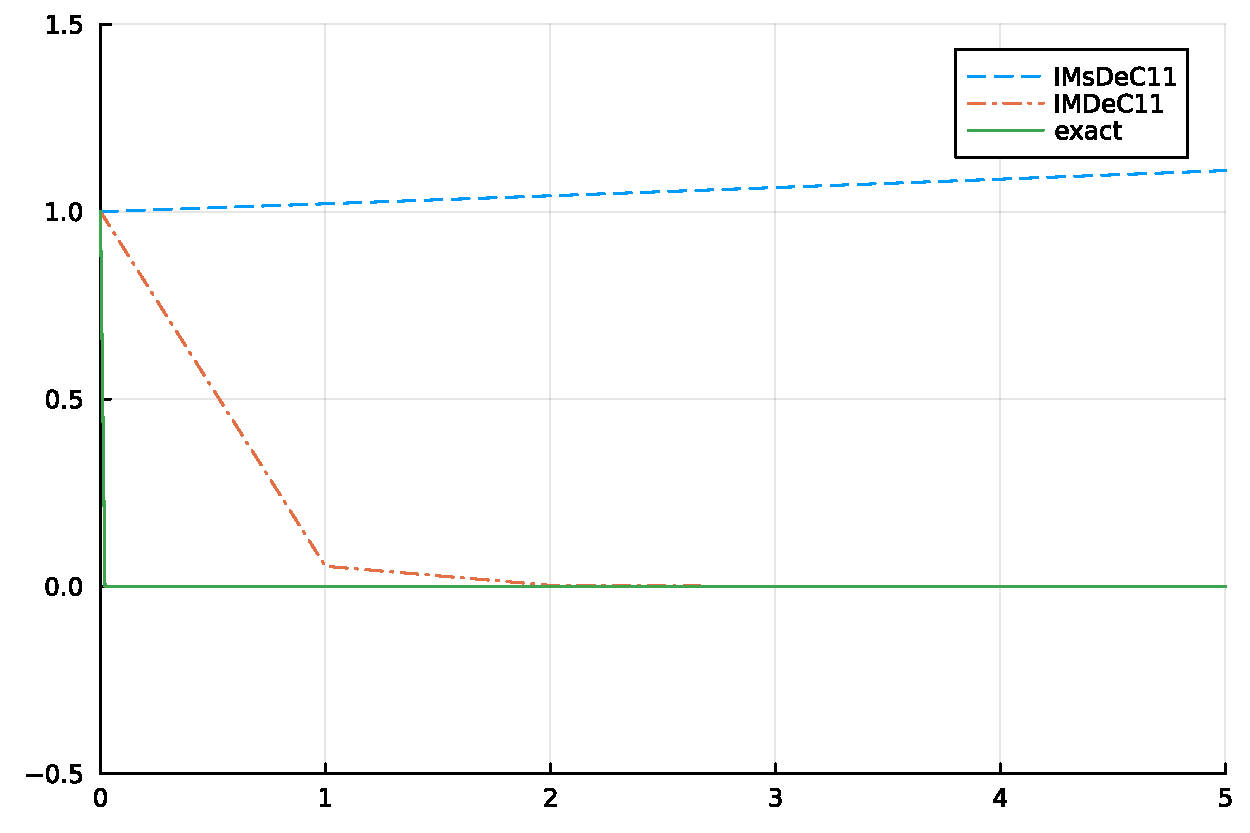
\includegraphics[width=\textwidth]{pdf/odepics/BspImsDeC/sol_ImsDeC11_GLB_stable10.pdf}
	\end{minipage}
	\begin{minipage}[t]{0.45\textwidth}
		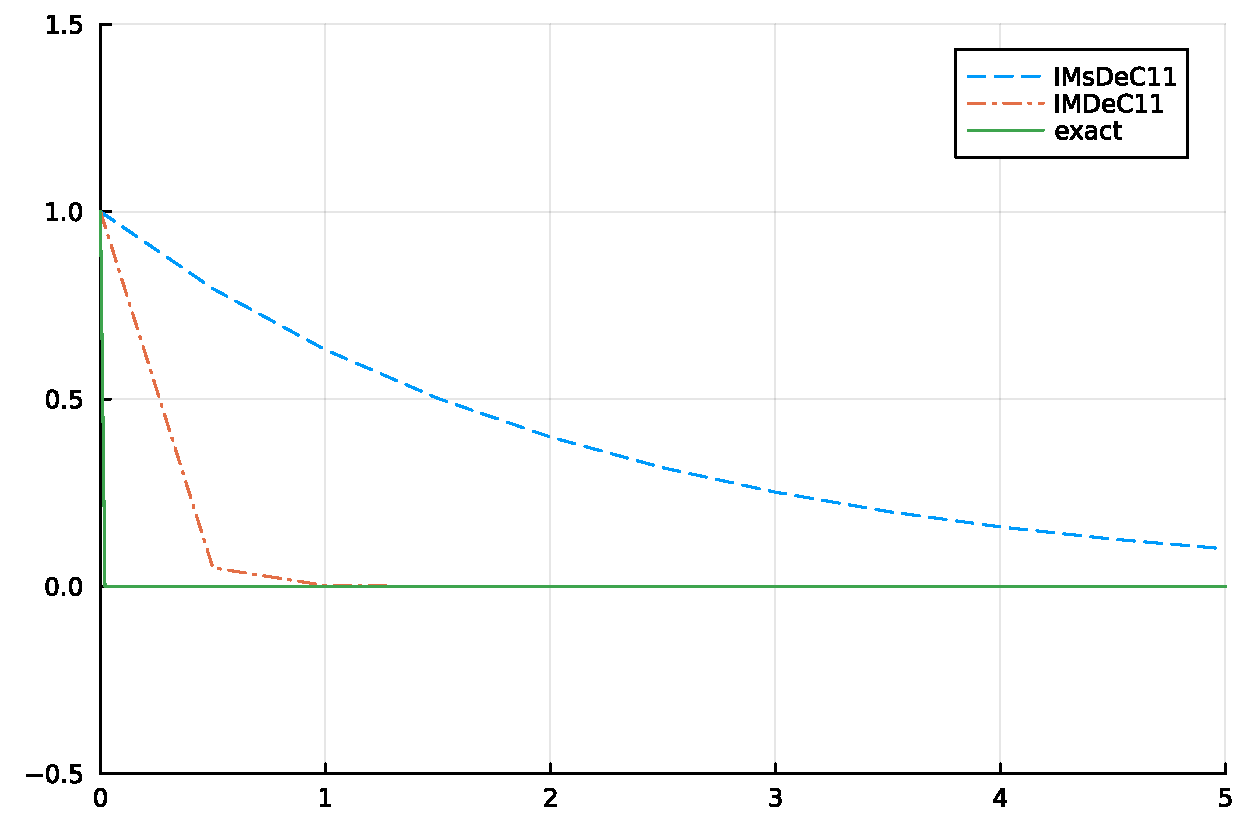
\includegraphics[width=\textwidth]{pdf/odepics/BspImsDeC/sol_ImsDeC11_GLB_stable20.pdf}
	\end{minipage}
	\caption{Solving \eqref{eq: ImsDeC_linear_scalar} using ImsDeC11 with $h=1$ (left) and $h=0.5$ (right)}
	\label{fig: exaImsDeC1}
\end{figure}

\begin{figure}
	\centering
	\begin{minipage}[t]{0.45\textwidth}
		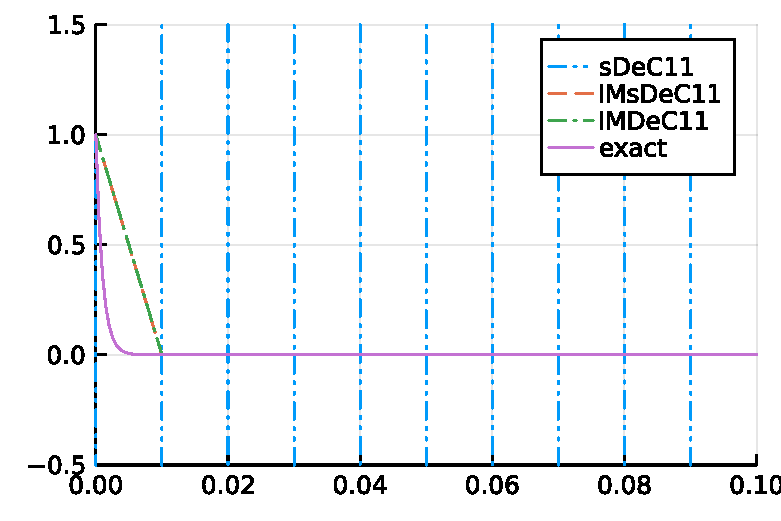
\includegraphics[width=\textwidth]{pdf/odepics/BspImsDeC/sol_ImsDeC11_GLB_stable1000.pdf}
	\end{minipage}
	\begin{minipage}[t]{0.45\textwidth}
		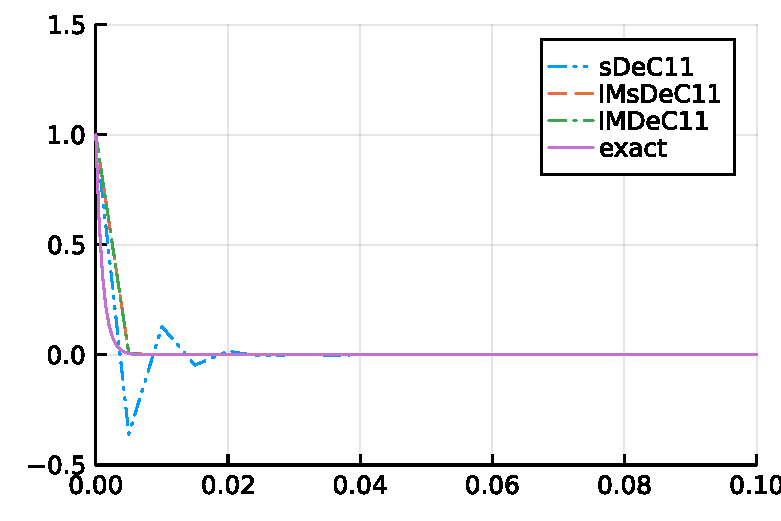
\includegraphics[width=\textwidth]{pdf/odepics/BspImsDeC/sol_ImsDeC11_GLB_stable2000.pdf}
	\end{minipage}
	\caption{Solving \eqref{eq: ImsDeC_linear_scalar} using ImsDeC11 with $h=0.01$(left) and $h=0.005$(right).}
	\label{fig: exaImsDeC2}
\end{figure}

Moving to a nonlinear example, we test the ImsDeC11 with Gauss-Lobatto nodes for the nonlinear ODE
\begin{equation}\label{eq: ImsDeC_nonlinear_scalar}
\partial_t y(t)=-10^6 \lvert y(t) \rvert \cdot y(t)+1, \quad y(0)=\frac{1}{\sqrt{10^6}}
\end{equation} 
and compare it again with the analogue ImDeC. We observe in Figure \ref{fig: exaImsDeC4} on the left that the ImDeC handles the stiff equation well, while the ImsDeC again has an unstable behavior for the step $h_1=1$. This coincides with the stability region because for our nonlinear equation, an equivalent to $\lambda$ could be roughly obtained by linearizing the equation, so that $\lambda:=-10^6\lvert y(t) \rvert \approx -10^6\cdot \frac{1}{\sqrt{10^6}}=-10^3$ and therefore  $z_1\approx-10^3\notin S$. Nevertheless, after refining to $h_2=0.5$ we have $z_2\approx -500$ and we expect again stability for the ImsDeC, which can be seen on the right of Figure \ref{fig: exaImsDeC4}.
The results of their explicit counterparts are not included in these Figures, because they diverge above $h=0.1$ and are therefore not comparable in the same Figure. \\
Summarized we can observe that the non-A-stable ImsDeC performs worse than the ImDeC for stiff applications, but may still be applicable up to a certain degree and gives better results for this type of equations than the explicit sDeC.

\begin{figure}[!h]
	\centering
	\begin{minipage}[t]{0.45\textwidth}
		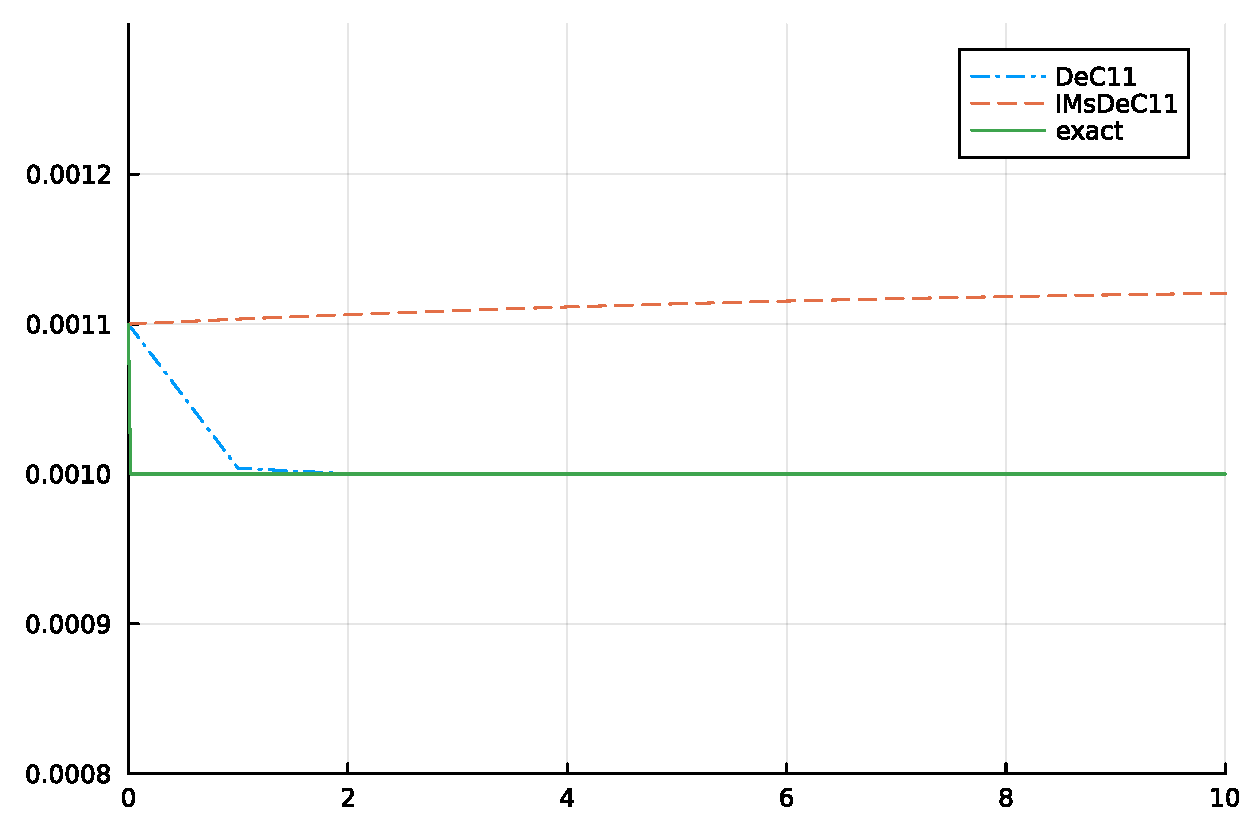
\includegraphics[width=\textwidth]{pdf/odepics/BspImsDeC/sol_ImsDeC11_GLB_nonlinear1.pdf}
	\end{minipage}
	\begin{minipage}[t]{0.45\textwidth}
		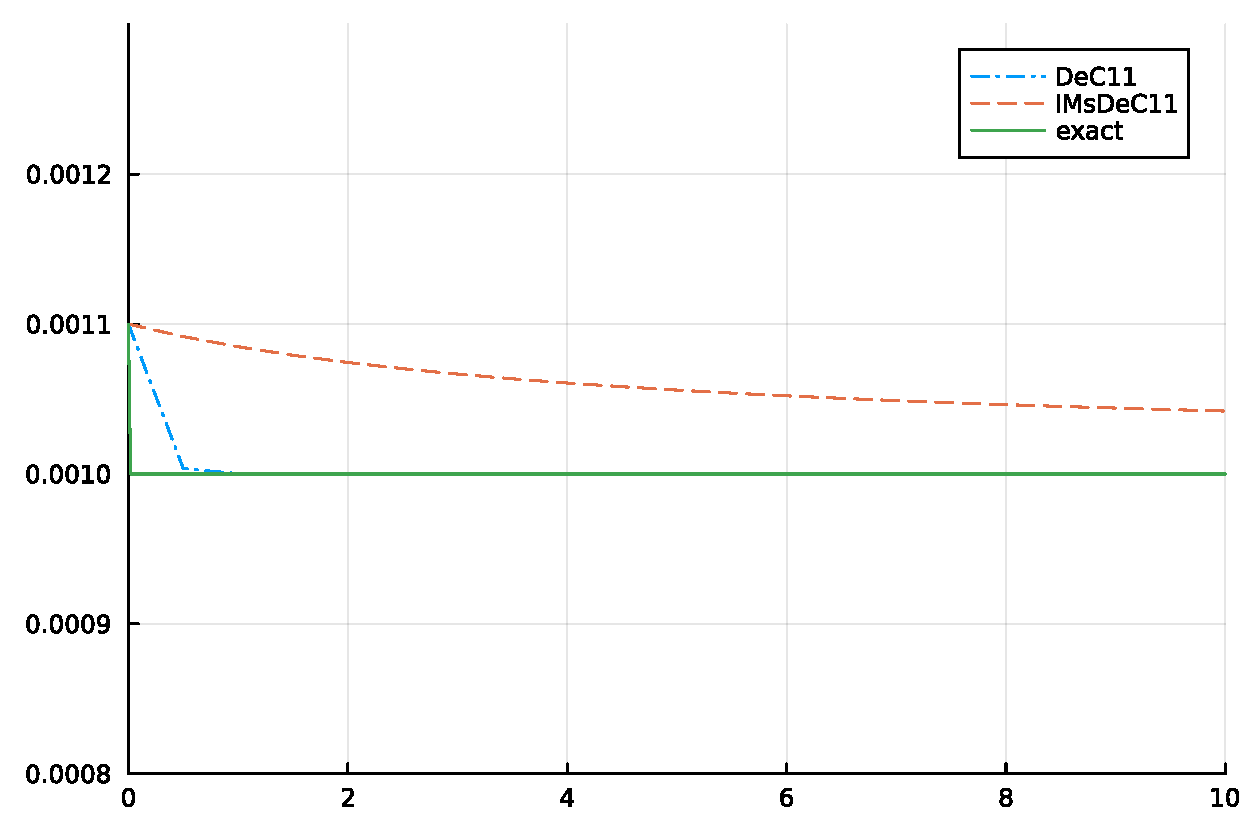
\includegraphics[width=\textwidth]{pdf/odepics/BspImsDeC/sol_ImsDeC11_GLB_nonlinear2.pdf}
	\end{minipage}
	\caption{Solving equation \eqref{eq: ImsDeC_nonlinear_scalar} using ImsDeC11 with $h=1.0$(left) and $h=0.5$(right).}
	\label{fig: exaImsDeC4}
\end{figure}

\subsubsection{A stiff, linear example for the IMEX methods}
We consider the second order ODE
\begin{equation}
\partial_{tt} y(t)=-2\partial_t y(t)-2501 y(t),\quad y(0)=1, \; \partial_y(0)=0,
\end{equation}
which can be rewritten as a system of ODEs
\begin{equation}\label{eq: ODE_linear_ImEx}
\begin{aligned}
\partial_t u_1(t)&=-2 u_1(t)-2501u_2(t), \quad &u_1(0)=1, \\
\partial_t u_2(t)&=u_1(t), &u_2(0)=0.
\end{aligned}
\end{equation}
The exact solution is given by 
\begin{equation*}
\vec{u}(t)=\left(\begin{array}{c}
y(t)\\
\partial_t y(t)
\end{array}\right)	=\left(\begin{array}{c}
\frac{1}{50}e^{-t}\left(\sin(50t)+50\cos(50t)\right) \\
-\frac{2501}{50}e^{-t}\sin(50t)
\end{array}\right),
\end{equation*}
i.e. we have a rapid oscillation and a slow transient part.
Therefore we seperate the right-hand side of \eqref{eq: ODE_linear_ImEx} by 
\begin{equation*}
F_I(\vec{u}(t))=\left(\begin{array}{c}
-2501 u_2(t)\\
u_1(t)
\end{array}\right), \quad 
F_E(\vec{u}(t))=\left(\begin{array}{c}
-2u_1(t)\\
0
\end{array}\right)
\end{equation*}
to treat $F_I$ implicitly and $F_E$ explicitly.\\
The numerical solutions for IMEX ADER, IMEX DeC and to comparison ADER are shown in Figure \ref{fig: exaImEx_linear}, all methods of order 5. As before, we observe stability for the IMEX methods while the explicit ADER does not converge towards the exact solution. 
A test with the other respective IMEX or pure explicit and implicit methods was done and gave similar results: the explicit analogues behaved as ADER, while the implicit did not differ heuristically from the IMEX methods.
\begin{figure}
	\centering
	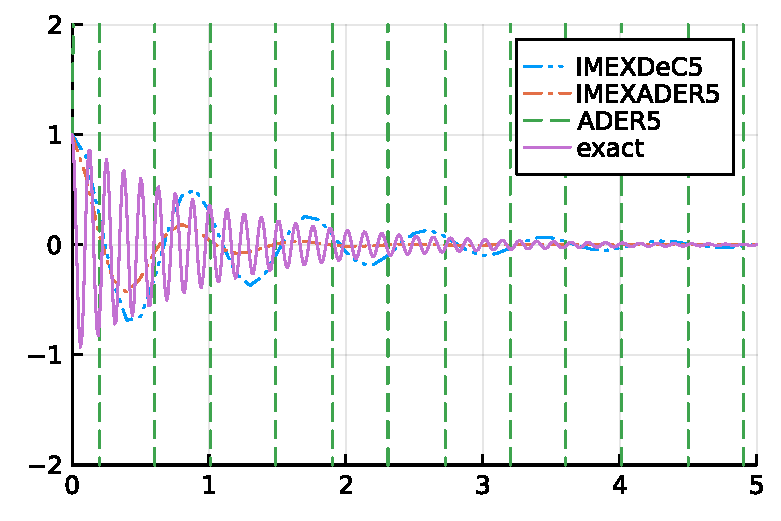
\includegraphics[width=0.6\textwidth]{pdf/odepics/Num_val/exa_ImEx_linear.pdf}
	\caption{Solving equation \eqref{eq: ODE_linear_ImEx} with different methods using equispaced nodes with $h=0.1$.}
	\label{fig: exaImEx_linear}
\end{figure}

%\subsubsection{The Robertson Problem} \todo{I would do Robertson or stiff linear only... }
%Now, we want to take a brief look on the famous Robertson problem, describing a chemical reaction. The underlying ODE is given by
%\begin{equation}\label{eq: RobertsonODE}
%\begin{aligned}
%\partial_t u_1(t) &=  \alpha u_2(t)u_3(t)-\beta u_1(t)\\
%\partial_t u_2(t) &=  \beta u_1(t)-\alpha u_2(t) u_3(t)-\gamma u_2(t)\\
%\partial_t u_3(t) &=  \gamma u_2(t)\\
%\end{aligned}
%\end{equation}
%with $\alpha = 10^4,\ \beta = 0.04$ and $ \gamma = 3\cdot 10^7$. It is known that explicit methods are able to solve this method for some seconds, but fail at larger time scales. For our methods, we provide some examples in the appendix~\ref{subsec:robertson_explicit}. 
%In Figure~\ref{fig: exaExRobertson_ord3_N=10}, the ODE is solved by the IMEX DeC, sDeC and ADER methods, respectively for order 3. We observe that these methods have no problem at all solving this larger time steps, even with only 20 time steps. \\
%For the Robertson problem we used exponential distributed timesteps \cite{offner2019arbitrary} and Gauss-Lobatto nodes for every method. Further variations in order, time steps and nodes are not included here, but were tested and observed respectively the numerical solutions of $u_2$ and they all coincide with the expectations.
%
%\begin{figure}
%	\centering
%	\begin{minipage}[t]{0.45\textwidth}
%		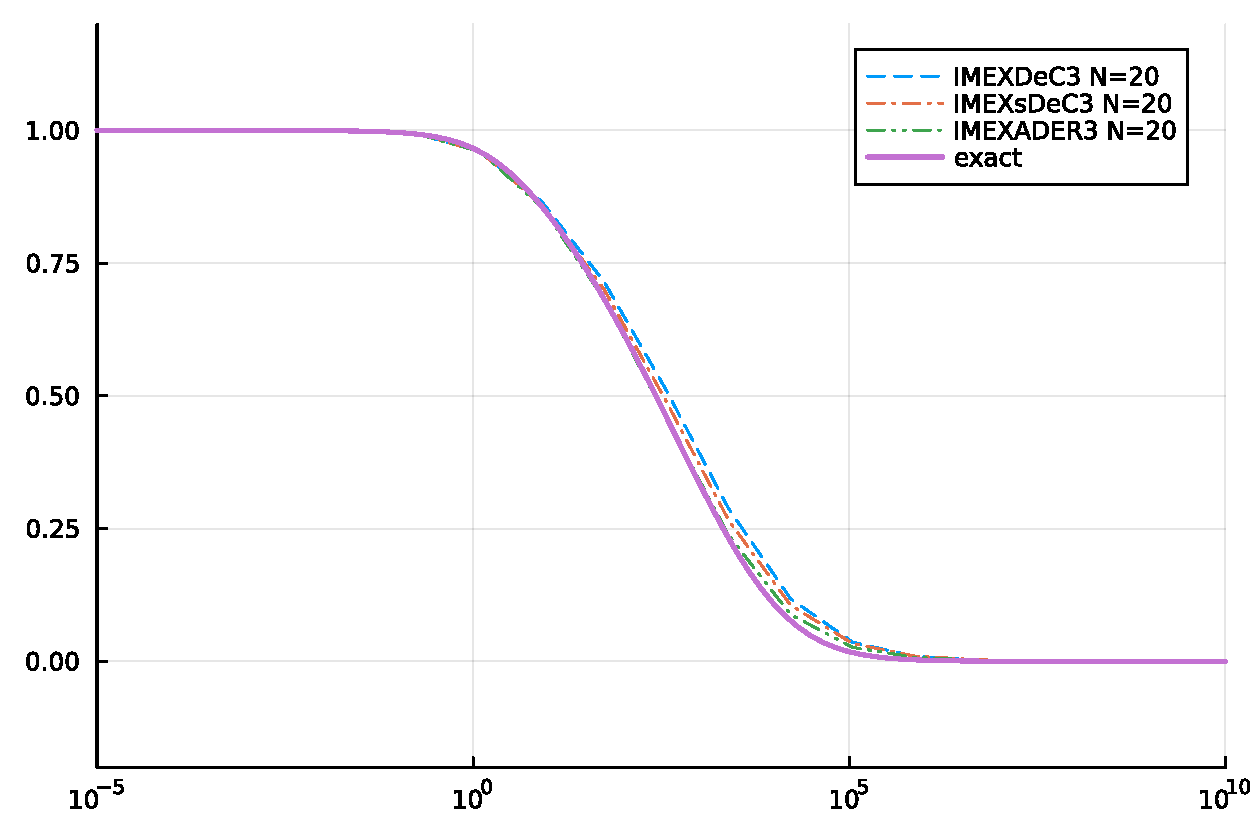
\includegraphics[width=\textwidth]{pdf/odepics/Num_val/IMrobertson_dim1_ord3_N=20.pdf}
%	\end{minipage}
%	\begin{minipage}[t]{0.45\textwidth}
%		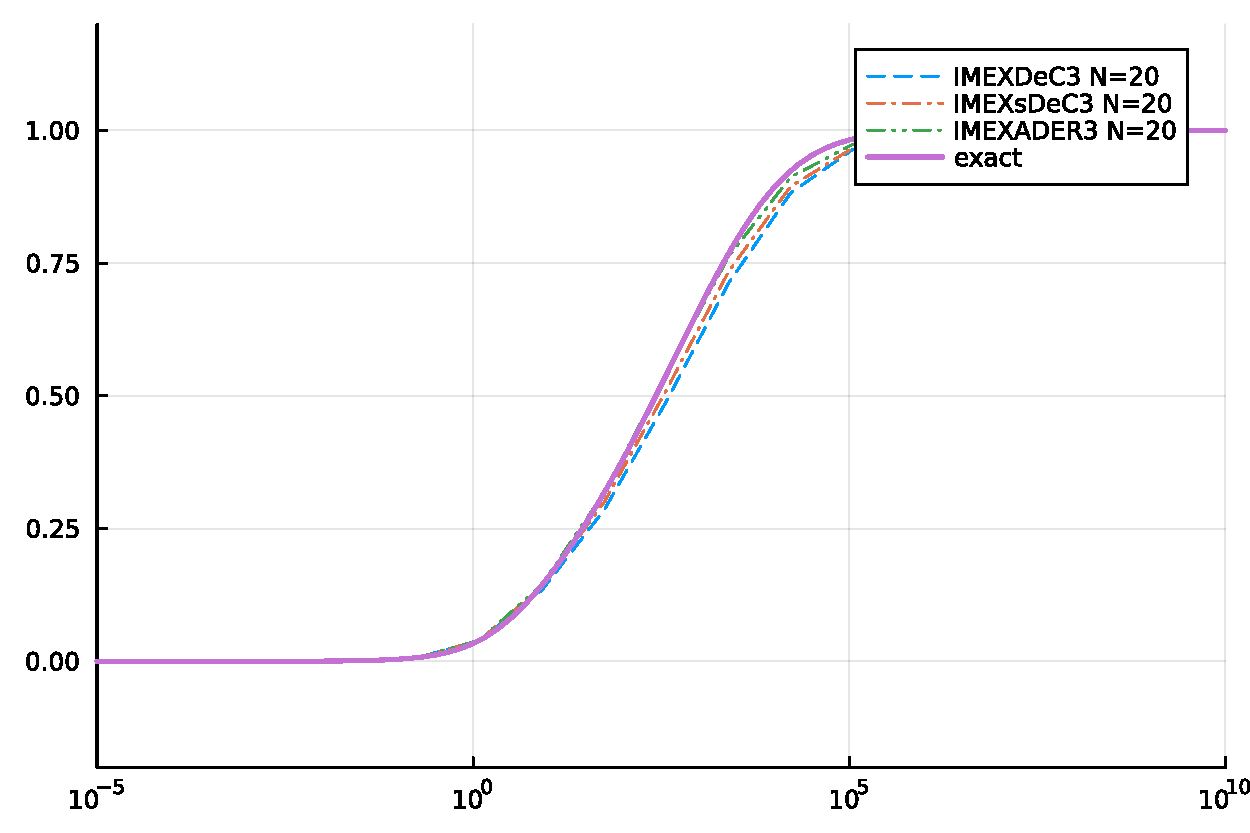
\includegraphics[width=\textwidth]{pdf/odepics/Num_val/IMrobertson_dim3_ord3_N=20.pdf}
%	\end{minipage}
%	\caption{Solving equation \ref{eq: RobertsonODE} using IMEX methods of order 3 with GLB nodes for $u_1$ (left) and $u_3$ (right).}
%	\label{fig: exaExRobertson_ord3_N=10}
%\end{figure}


\subsection{PDE tests}
A couple of tests showing stability instability.

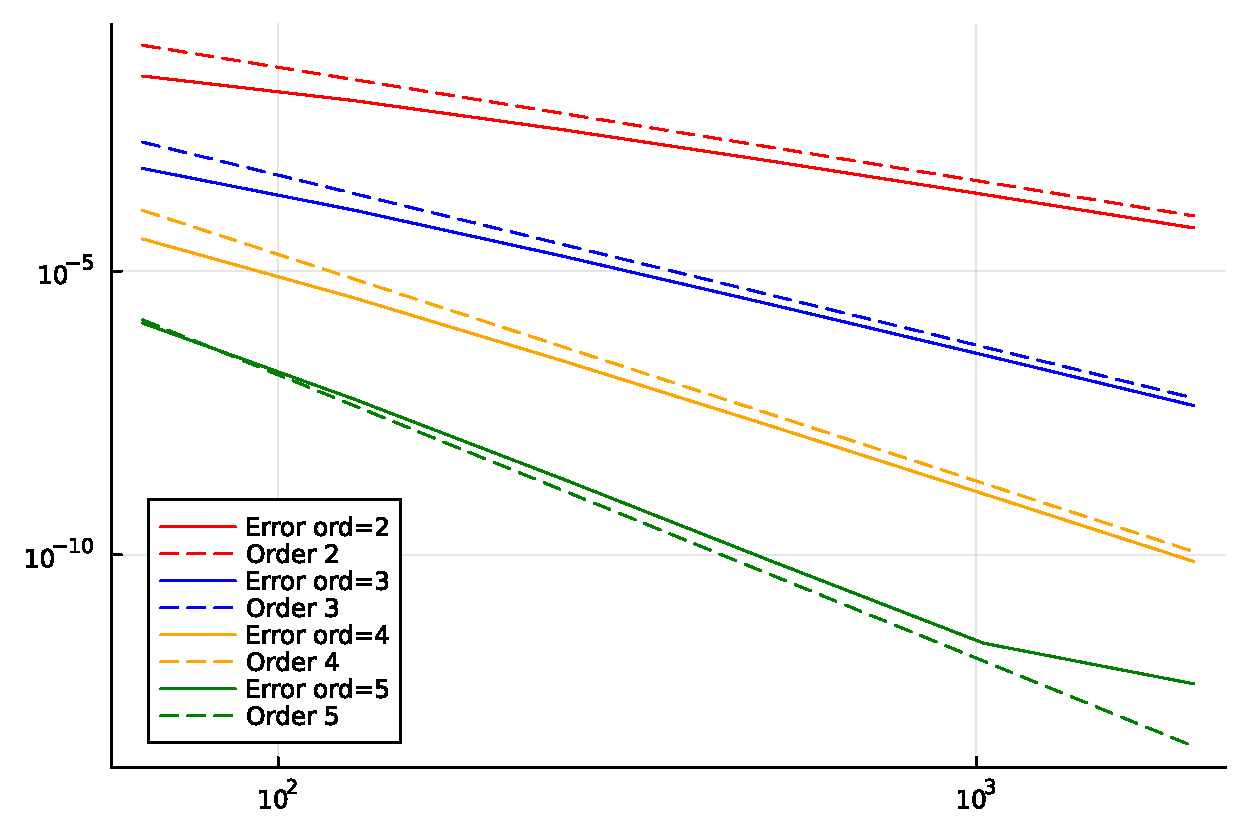
\includegraphics[width=0.32\textwidth]{pdf/pdepics/numerics/DeC_errors.pdf}
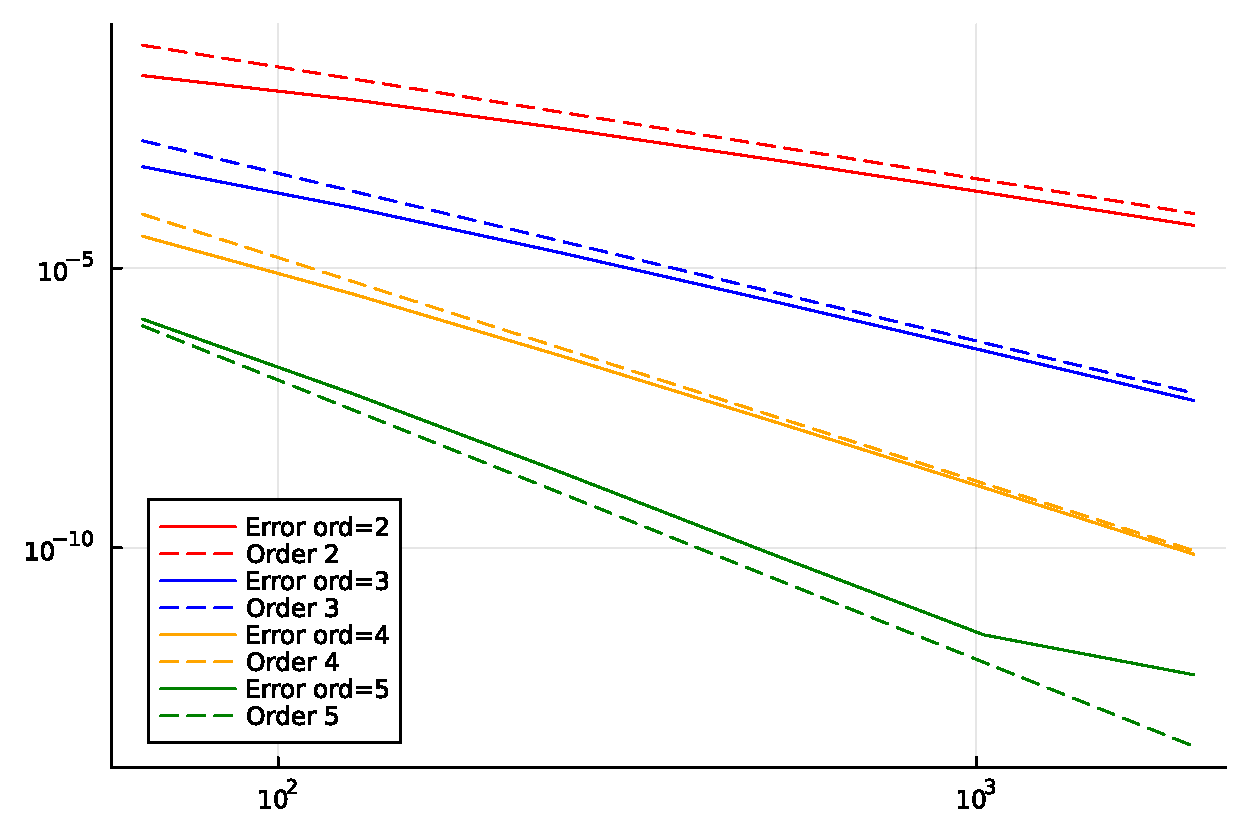
\includegraphics[width=0.32\textwidth]{pdf/pdepics/numerics/sDeC_errors.pdf}
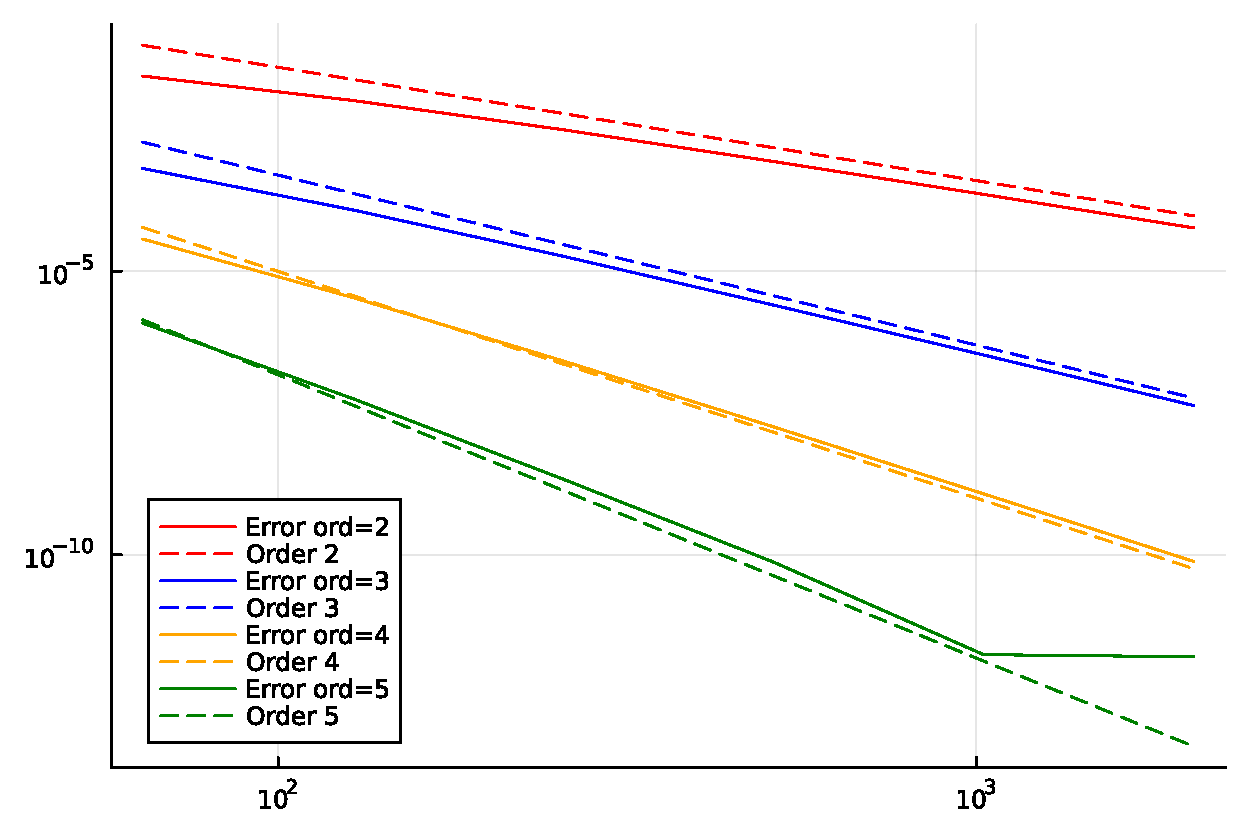
\includegraphics[width=0.32\textwidth]{pdf/pdepics/numerics/ader_errors.pdf}
